\section{Turbulent Flows}

In the realm of engineering, there is often a need to predict fluid flow behavior in and around engineered products.
These situations can range from simulating the flow around an airplane to simulating the flow through laptop cooling systems.
Computational Fluid Dynamics (CFD) is the field of study that involves using computers and complex numerical analysis techniques to solve the non-linear Navier-Stokes equations on the flow domain of interest.
As computational capabilities have increased over the past few decades, so has the reliance on the predictive capability of CFD simulations. 

CFD simulations are made more difficult due to turbulence.
The range of length and time scales that need resolving through spatial and temporal discretization makes it computationally intractable to solve precisely, i.e., without simplifying models.
Turbulence plagues most flows of engineering interest.
The difficulty in solving these flows has paved the way for developing a hierarchy of solution techniques that trade computational cost for prediction accuracy. 

\begin{figure}
    \center
    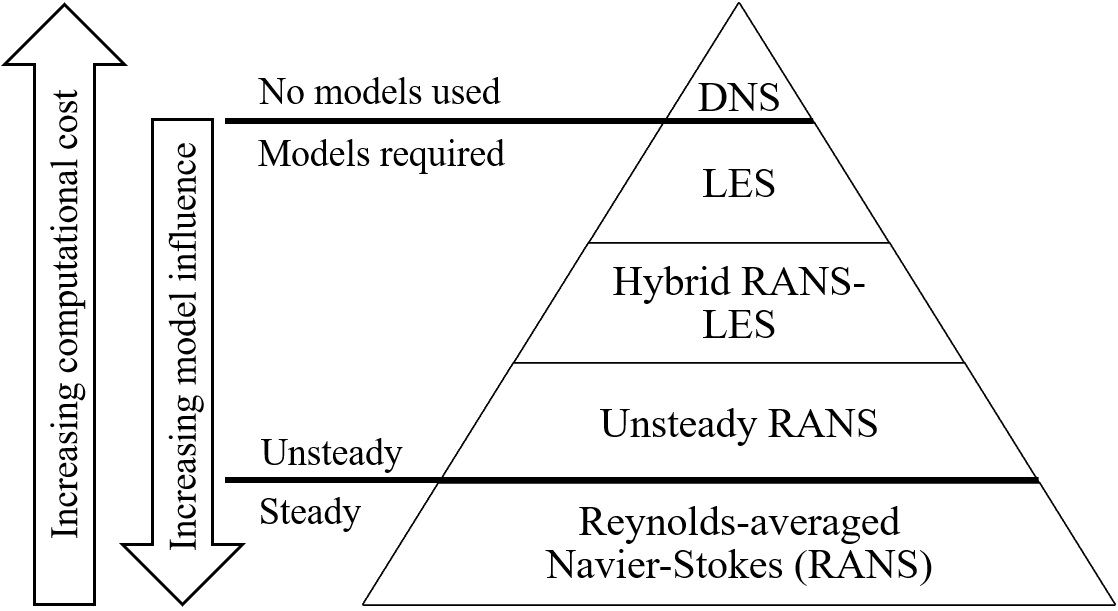
\includegraphics[width=0.75\textwidth]{suthesis/images/solution_heirarchy_simple.png}
    \caption{Hierarchy of CFD solution techniques in order of increasing computational cost and decreasing model influence. \label{fig:cfd_types}}
\end{figure}

Figure \ref{fig:cfd_types} presents this hierarchy in the form of a pyramid.
Sitting at the top of this pyramid are Direct Numerical Simulations or DNS.
These calculations do not employ any mathematical models and resolve all spatial and temporal time scales to give an exact reproduction of the fluid behavior.
These time-varying (unsteady) simulations are computationally expensive and memory intensive.
At the time of writing, DNS calculations are only possible at low Reynolds numbers and for simple geometries such as flat plates \cite{hoyas_reynolds_2008}, and channels \cite{laval_marquillie_dns_channel,marquillie_instability_2011}.
These limitations disqualify the use of DNS, in its current state, for practical engineering applications. 

Below DNS, in Figure \ref{fig:cfd_types}, lie Large Eddy Simulations (LES) and Hybrid RANS-LES simulations.
These unsteady simulations resolve some, but not all, of the scales of turbulence.
Unresolved time and length scales are modeled using simplifying assumptions \cite{pope_2000}.
These solution methodologies allow for the fine-tuning of the desired influence of simplifying models through the chosen level of spatial and temporal discretization.
They are in the process of being adopted by industry for specific use cases such as performance predictions for high-lift configuration aircraft \cite{rumsey2019overview}, or engine simulations. 

The pyramid's base represents the most widely used method in the industry, Reynolds-averaged Navier-Stokes (RANS) simulations.
These simulations suffer the most from modeling inaccuracies.
They assume that the flow is steady (no time-dependent variation in the flow features) and require simplifying turbulence models that aggregate the effects of the turbulent eddies that would be present in the flow.
These simplifications significantly reduce the computational cost but inhibit the flow features that the simulations can capture.
While its unsteady counterpart can resolve some of the time variations of the flow, turbulence modeling is still required, affecting prediction accuracy.
Steady RANS simulations are very computationally efficient and can be used for expensive undertakings such as iterative aerodynamic shape optimization \cite{lyu2015aerodynamic}, and aircraft database generation \cite{wendorff_combining_2016}.
This chapter will focus on quantifying the uncertainties injected by turbulence models employed in RANS simulations. 